%
% File: chap01.tex
% Author: Victor F. Brena-Medina
% Description: Introduction chapter where the biology goes.
%
\let\textcircled=\pgftextcircled
\chapter{Active Matter}
\label{chap:activeMatter}




\initial{A}ctive matter refers to systems comprised of active units, where each unit is able to consume energy from the environment for self-propulsion.
 %an object with some broken isotropy; time reversal is also broken.
 In systems such as these, the injection of energy at the level of the individual, and the subsequent conversion of energy to mechanical motion, drives the system out of equilibrium \cite{ramaswamy2017}. The self-propulsion of these individual active units causes two symmetry breaking phenomena: a breaking of isotropy \cite{marchetti2013} and a breaking of time-reversal symmetry \cite{obyrne2022a}.
This definition of active matter is deliberately general and can therefore include many systems spanning a large range of length scales: from microscopic systems such as swimming bacteria \cite{zhang2010b}, actin filaments \cite{schaller2010}, and self-propelling colloids \cite{theurkauff2012}; to macroscopic systems including fish \cite{gautrais2009}, birds \cite{cavagna2014} and even human crowds \cite{bottinelli2016} (Fig. \ref{fig:AMcollage}).

\begin{figure*}
	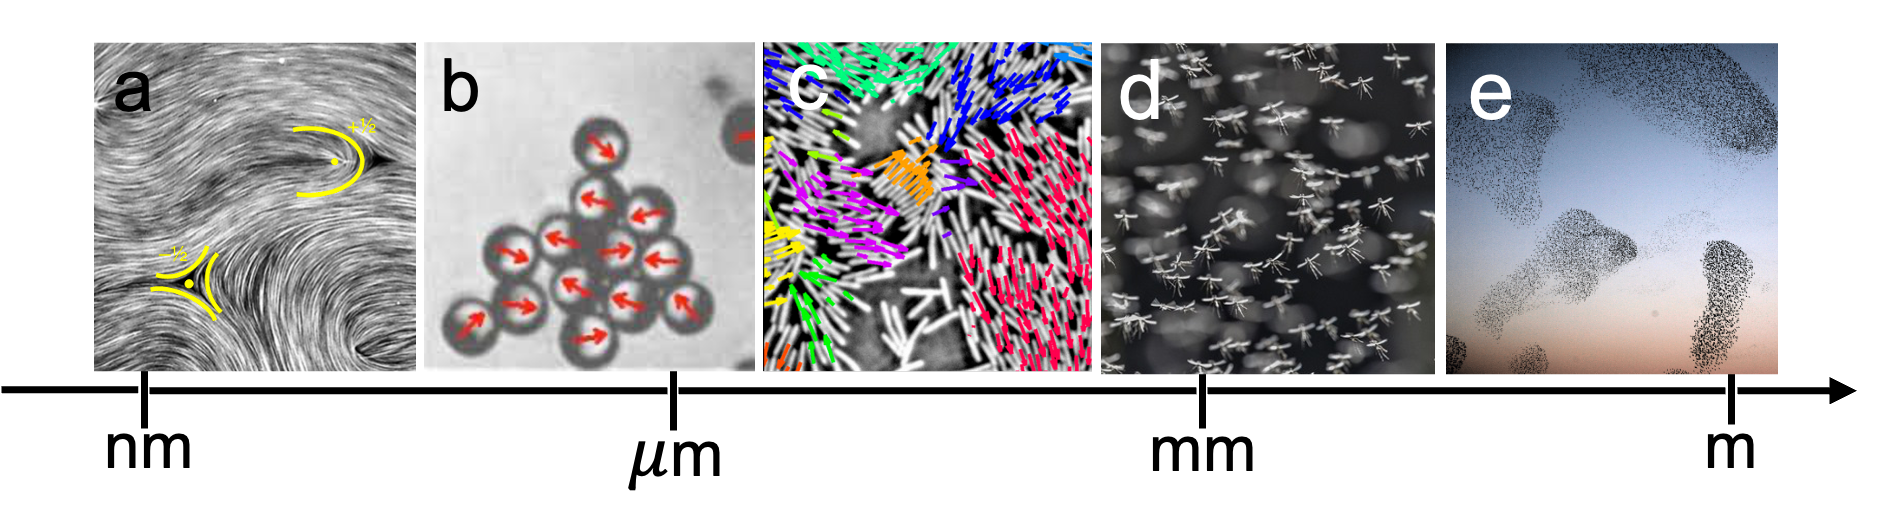
\includegraphics[width=\linewidth]{chapters/activeMatter/figsActiveMatter/figAMcollage.png}
	\caption[Active matter across multiple lengthscales]{Active matter across multiple lengthscales. \textbf{a} Turbulence in actin tissues. \textbf{b} Clustering of self-propelling colloids without attraction. \textbf{c} Alignment in swimming bacterial colonies. \textbf{d} Swarming in midges. \textbf{e} Bird flocks undergo collective motion.}
	\label{fig:AMcollage}
\end{figure*}


When these active units come together to interact as an ensemble, we observe the emergence of rich and complex dynamical phenomena unique to non-equilibrium systems such as: collective motion in bacteria, fish and birds \cite{vicsek2012}; non-equilibrium separation in self-propelled colloids \cite{cates2015}; and turbulence in baths of molecular motors \cite{doostmohammadi2018}. 
The vibrant behavioural phenomenology of these systems has attracted many to work in this rapidly developing field, where fundamental physics seemingly underlies the motion and interactions of living systems on multiple lengthscales. These systems have provided a new lens through which to study a wide-range of topics across many disciplines including: non-equilibrium statistical mechanics \cite{cates2012,ramaswamy2017}, biology \cite{viswanathan2011}, soft matter physics \cite{marchetti2013,bechinger2016a}, engineering \cite{brambilla2013}, and medicine \cite{wang2012,tarantola2019}.

This chapter is structured as follows: in section \ref{section:activeMatter:models} we begin with an introduction to the physics governing active particle motion. This is then followed in section \ref{section:activeMatter:phenom} by a review of the main phenomenological behaviours that arise through the bulk interactions of active matter. With this baseline established, we narrow our focus to the specifics of this thesis: active matter confined in complex environments (section \ref{section:activeMatter:confinement}); and finish with section \ref{section:activeMatter:janus}, on the self-propulsion mechanisms for Janus colloids.


\section{Describing the dynamics of active systems}
\label{section:activeMatter:models}

Active matter can describe a wide range of dynamical systems and the resultant phenomenology displayed in these active systems is dependant on the class that each active unit belongs to. These \textit{classes} (Fig.  \ref{fig:AMclasses}) can be selected through the following groupings: a self-propelling particle can be described as \textit{polar}, meaning that as well at it's position, it also possesses an intrinsic directional component describing the orientation of the self-propulsion. Systems of polar active units with an alignment mechanism express the phenomena of collective motion (or flocking); demonstrating polar or nematic alignment.
In systems of active polar particles with \textit{scalar} interactions, meaning pair-wise potentials that are dependant on the particle positions, not the orientations. These systems can undergo a non-equilibrium phase separation under certain conditions, and in the absence of attractive interactions. 
The final class regards dipolar particles with a nematic alignment. These systems exhibit active nematic \textit{turbulence}, involving the dynamical evolution of  topological defects. Also known as \textit{active nematics}, these systems are the focus of a vibrant field of research \cite{doostmohammadi2018,giomi2015,alert2020}, but lie outside the scope of this work. The mesoscale active matter systems that are the focus of this work are best described as polar particles with scalar interactions, and the dynamics of these systems are described with active Brownian particle models. In this section we detail the models that best capture this behaviour and their characteristic dynamical behaviour.


\begin{figure*}
	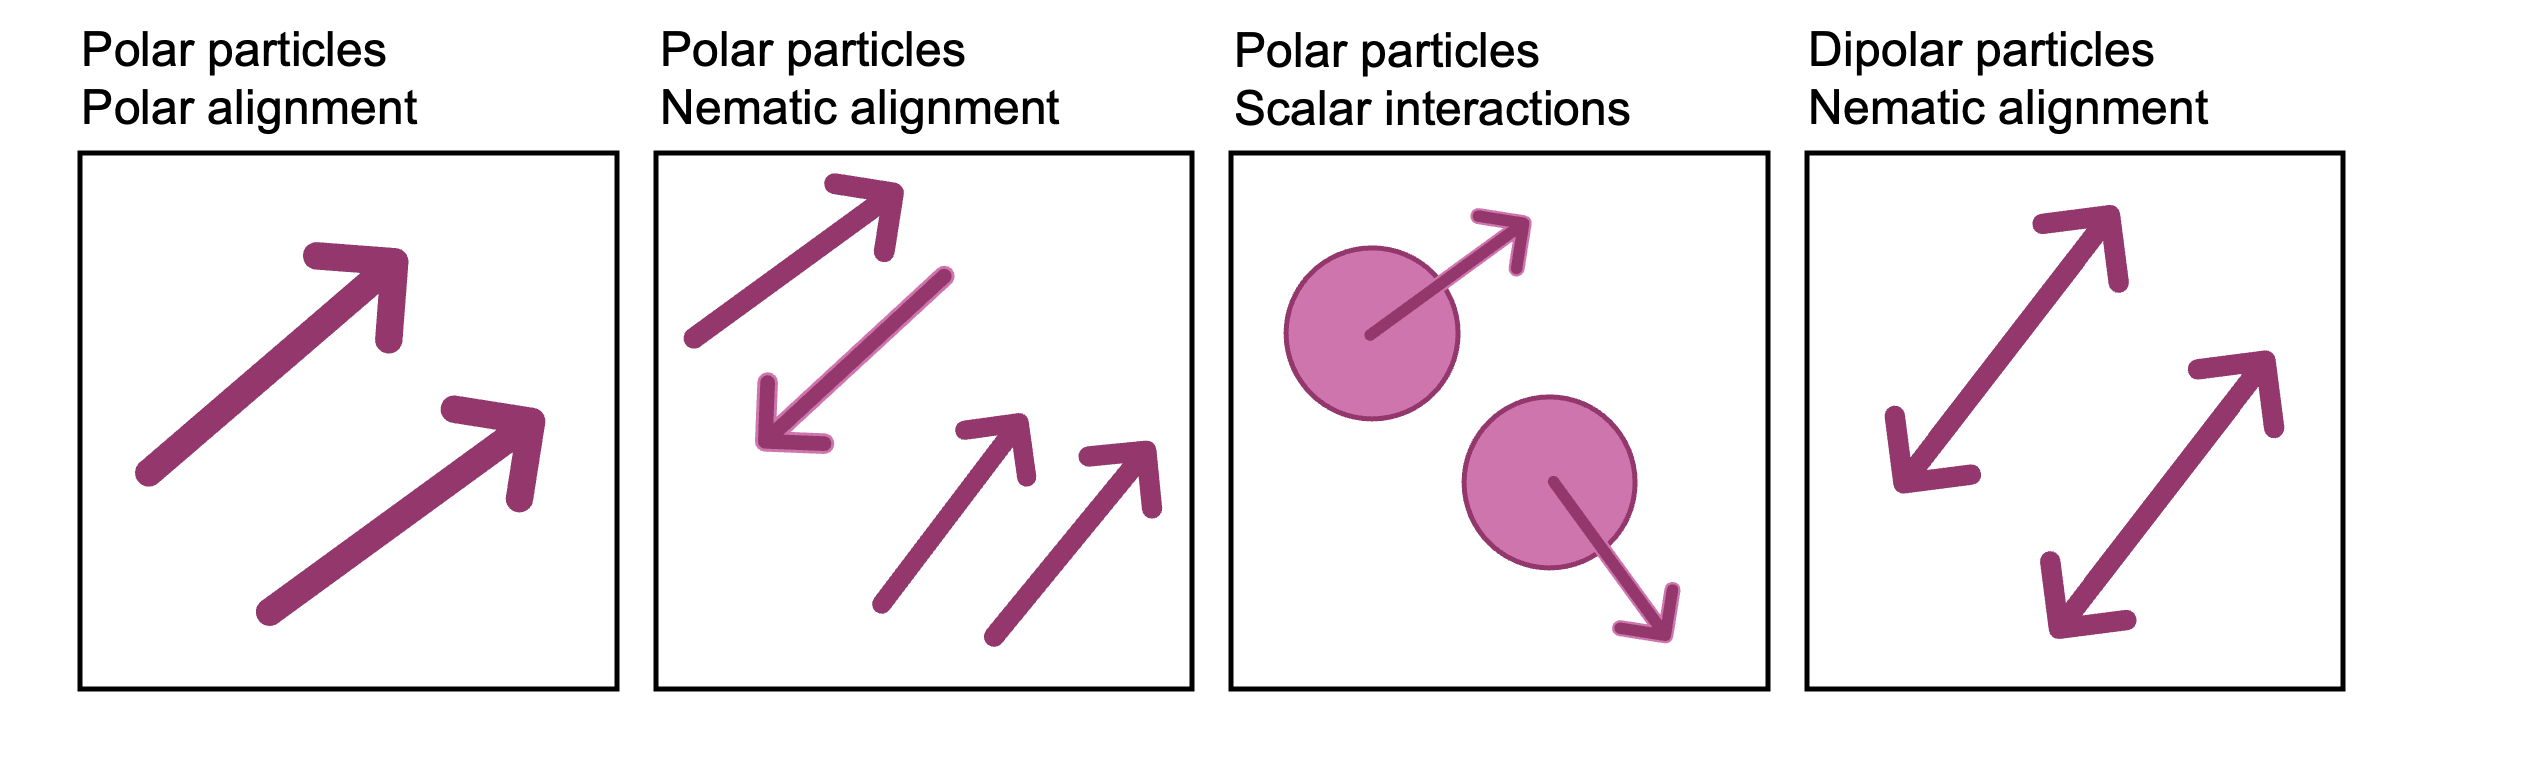
\includegraphics[width=0.9\linewidth]{chapters/activeMatter/figsActiveMatter/figParticleType}
	\centering
	\caption[Classes of active matter]{Four \textit{classes} of active matter. The interactions of particles within each class bring out unique behavioural phenomena.}
	\label{fig:AMclasses}	
\end{figure*}


In the most simple terms, an active particle of mass $m$ can modelled with the following equation of motion:


\begin{equation}
	m \ddot{\mathbf{r}}=-\gamma \dot{\mathbf{r}}+\mathbf{F}_{\mathrm{p}}(t)-\nabla V(\mathbf{r})+\sqrt{2 \gamma^{2} D} \mathbf{\xi}(t),
    \label{eq:ABP3D}
\end{equation}

\noindent where the vector $\mathbf{r}$ defines the particle position, $\gamma$ is the damping coefficient, $\mathbf{F}_{\mathrm{p}}$ is the active propulsion force, $V(\mathbf{r})$ refers to the particle interaction potential, $D$ is the diffusion coefficient, and $\mathbf{\xi}$ is a Gaussian noise term representing thermal fluctuations that  promote diffusion.

In equilibrium systems energy is both injected and dissipated by the surrounding fluid. Thermal fluctuations of this fluid result in an injection of energy from the stochastic force $\sqrt{2 \gamma^{2} D} \mathbf{\xi}(t)$, a force that is in turn balanced by friction in the form of the dissipative force $-\gamma \dot{\mathbf{r}}$. This balancing of forces in equilibrium fluids is the fluctuation-dissipation theorem:

\begin{equation}
	D = k_B T / \gamma ,
\end{equation} 

\noindent where $k_B$ is the Boltzmann constant. 

It is through the propulsion force  $\mathbf{F}_{\mathrm{p}}$ that this description is driven out of equilibrium. The addition of this term introduces an irreversible injection of energy at the individual particle level in the form of a time-dependent, non-conservative force. The source of this energy will change depending in the active system: for bacteria this derives from the metabolism of food into ATP driving flagella or other swimming apparatus; for self-propelling colloids this energy may come from an external AC field that generates asymmetric ionic flows around the particle surface. Since these energy sources are independent from the thermal fluctuation and dissipation of the surrounding solvent, the balance is no longer satisfied and the system is driven out of thermal equilibrium \cite{obyrne2022a}. 





Active matter systems on mesoscopic lengthscales exist within fluids where viscous forces dominate over inertial forces. The ratio of these forces can be related via the Reynolds number:

\begin{equation}
	Re = \frac{u L}{\eta}, 
\end{equation}

\noindent where $u$ is the fluid velocity, $L$ is the characteristic dimension of the environment, and $\eta$ is the kinematic viscosity. For systems with active units on sufficiently small lengthscales to be subject to Brownian motion, the corresponding Reynolds number $Re<<1$ \cite{purcell2016}. Aside from a handful of studies interested in the role of inertia \cite{liao2021,nguyen2022,chatterjee2021}; the contributions from inertial forces are generally neglected, and these systems can be described with the following equation of motion:

 
\begin{equation}
    \dot{\mathbf{r}}=\mathbf{v}_{p} +\beta D_{T}\mathbf{F} +\sqrt{2D_{T}}\boldsymbol{\xi}_{T}.
    \label{eq:ABP3D_r}
\end{equation}

\noindent Here, $\mathbf{v}_p$ defines the velocity deriving from the self-propulsion force. $\beta = 1/k_B T$, $D_T$ is the translational diffusion coefficient, $\mathbf{F}$ is the external force, and $\boldsymbol{\xi}_{T}$ is a Gaussian white noise term, where $<\boldsymbol{\xi}_T>=0$. This equation of motion provides a general description of active dynamics, however in practise this model is further specialised towards a more phenomenological description through three standard models: active Brownian motion, run and tumble dynamics, and the active Ornstein-Uhlenbeck process. The primary difference in these models is in their description of the self-propulsion velocity $\mathbf{v}_p$. 



\begin{figure*}
	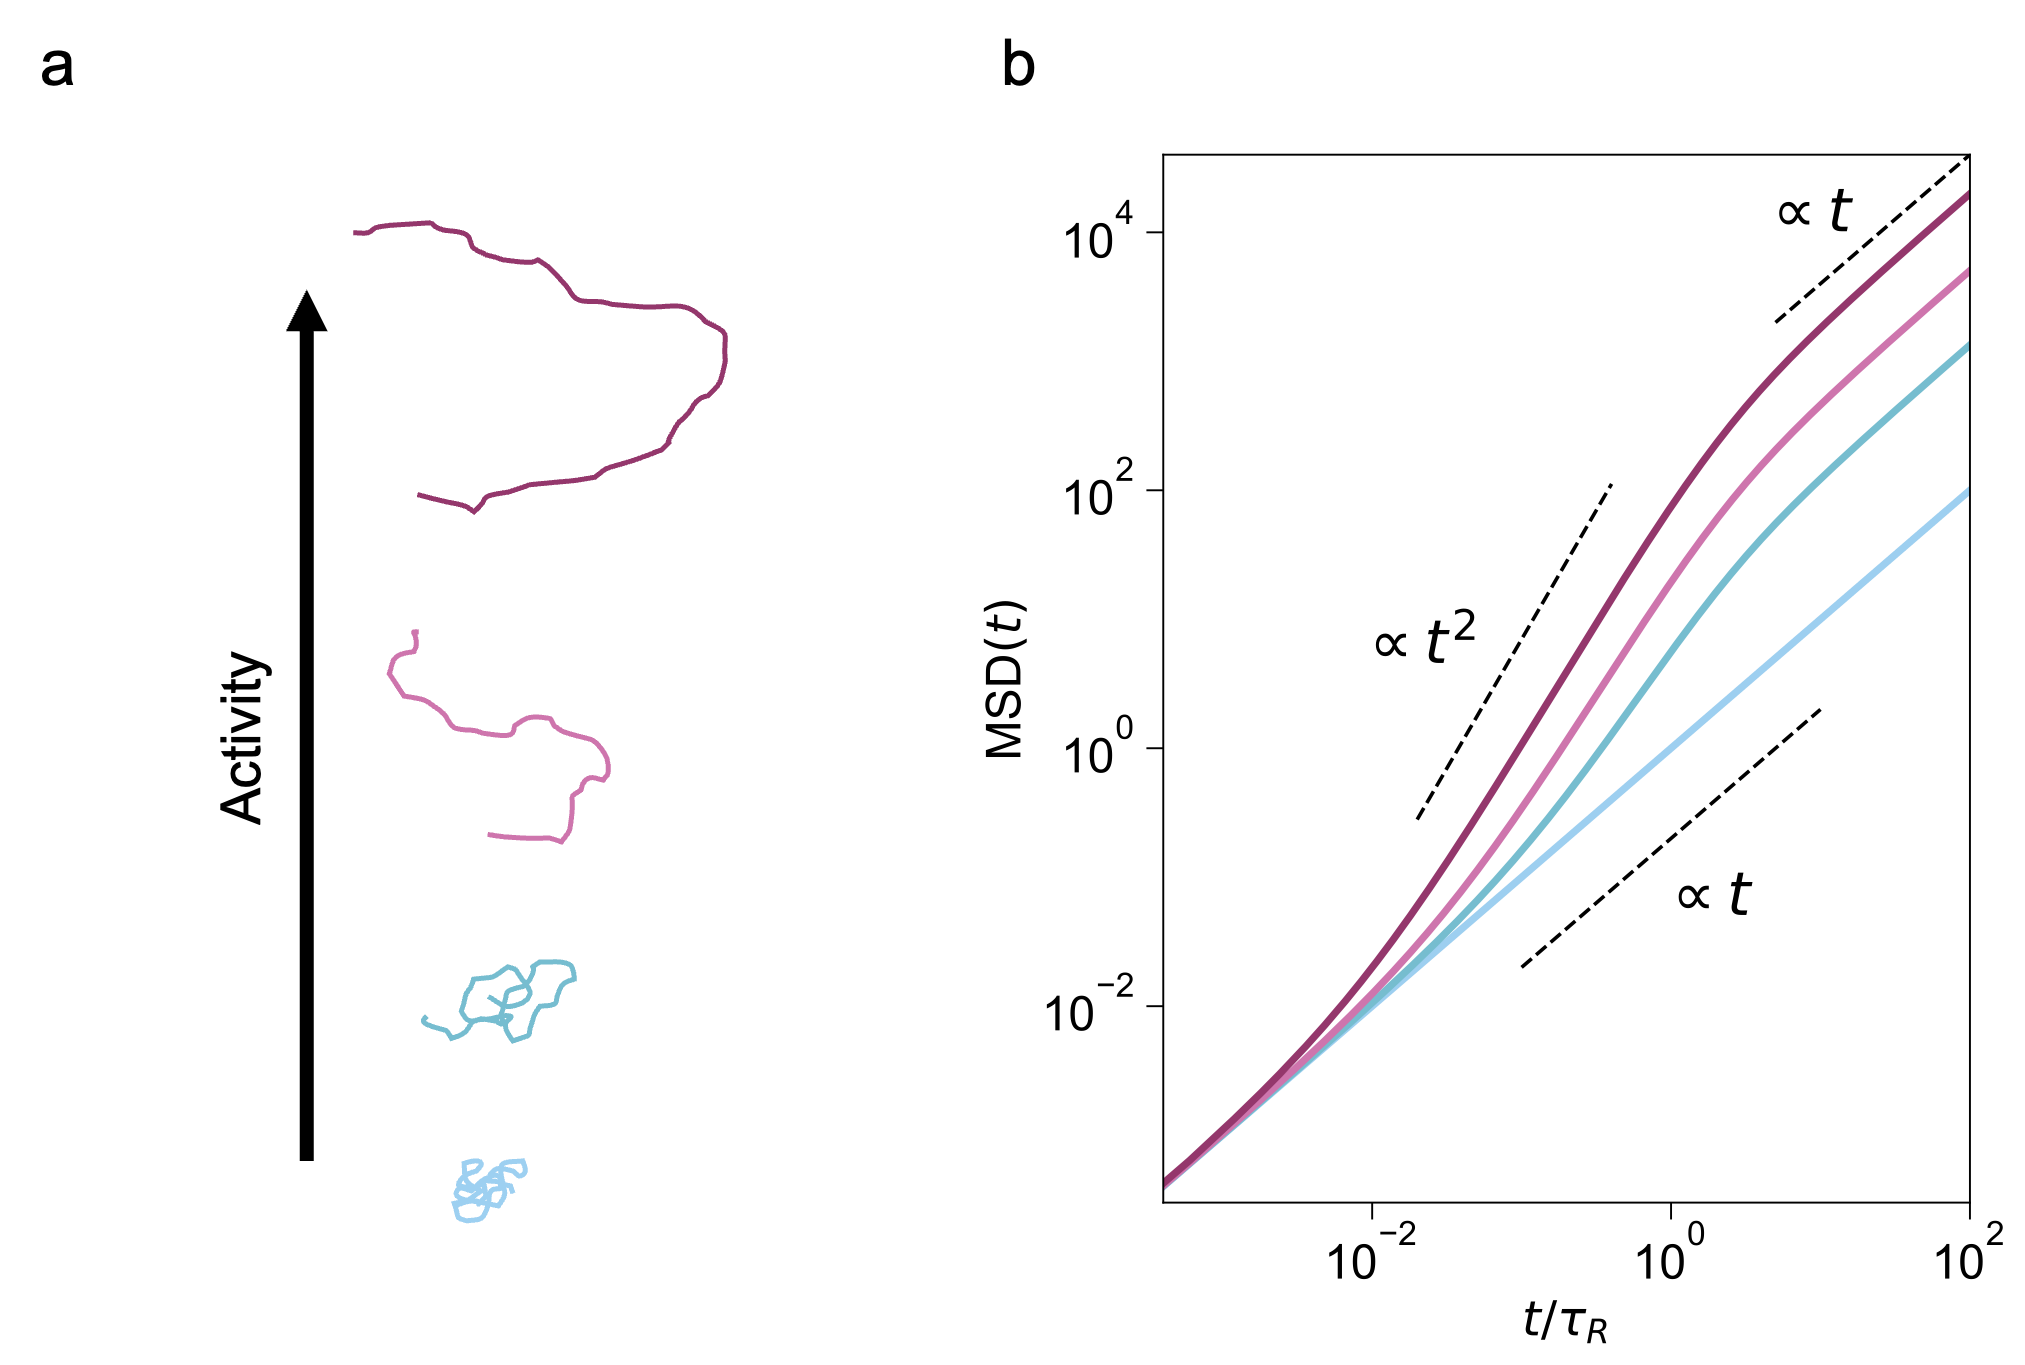
\includegraphics[width=\linewidth]{chapters/activeMatter/figsActiveMatter/fig3DabpMSD.png}
	\caption[Typical dynamics of active Brownian particles.]{\textbf{a} Schematic representation of four active Brownian particles of increasing activity. \textbf{b} Mean square displacement of active Brownian particles in 3D. Activity increases from the passive case (blue) to the most active (purple). The ballistic regime occurs over the timescale of $\tau_R$, during which the MSD $\propto t^2$. At long-times, the behaviour is diffusive with a higher effective diffusion: MSD $\propto t$.}
	\label{fig:ABP_example}
\end{figure*}

\textit{Active Brownian motion --- } this is one of the simplest and most extensively studied models of active matter. In these systems the self-propulsion velocity $\mathbf{v}_p = v_p \mathbf{e}$, where the magnitude of the velocity $v_p$ is constant, and the orientation $\mathbf{e}$ undergoes rotation diffusion according to:


\begin{equation}
    \dot{\mathbf{e}}=\sqrt{2D_{R}}\boldsymbol{\xi}_{R} \times \mathbf{e}.
    \label{eq:ABP3D_e}
\end{equation}

\noindent Here $D_R$ is the rotational diffusion coefficient and $\boldsymbol{\xi}_{R}$ is an independent Gaussian white noise vector, where $<\boldsymbol{\xi}_R>=0$. 
The direction of the self-propulsion will change as a result of thermal rotational diffusion over the timescale the rotational diffusion time: $\tau_R = 1 \ / \ 2D_R$ \cite{wysocki2014}.
In Fig. \ref{fig:ABP_example}a we show schematic trajectories of active Brownian particles in 2D for various active velocities $v_p$ in an unbounded and homogeneous environment. On short time-scales the trajectories are dominated by directed motion, and as dynamics progress this directed motion becomes randomised as the orientation changes with rotational diffusion. For active Brownian particles, the mean square displacement (MSD) has been determined analytically \cite{howse2007}, and in three-dimensions takes the form:

\begin{equation}
	\textrm{MSD} (t) = 6 D_{T} t+2 \tau_{R}^{2} v_{p}^{2}\left(t/\tau_{R}+e^{-t /\tau_{R}}-1\right).
	\label{eq:MSD_3D}
\end{equation}


\noindent Fig. \ref{fig:ABP_example}b plots this MSD for passive particles and active Brownian particles at a range of propulsion velocities. On very short timescales, where $t << \tau_R$ the contribution of the second term is negligible and the particles behave diffusively as MSD = $6D_T t$, this has been observed for active colloids at small propulsion velocities \cite{zheng2013a}. Over longer times scales, on the order of the rotational diffusion time ($t \approx \tau_R$), the particles enter a ballistic regime, where motion is highly directed: $\textrm{MSD}(t) = 6D_T t + 2v^{2}_{p}t^2$. At long times ($t >> \tau_R$), rotational diffusion of the direction of the self-propulsion acts to randomise the active contributions to the particle displacement. As a result of this, active particles move diffusively on average in the long time regime with an effective diffusion coefficient $D_\textrm{eff} > D_T$.




\textit{Run and tumble dynamics ---} this model was created to describe the motion of bacteria. Certain bacteria such as \textit{Escherichia coli}, swim through their environment in a sequence of "runs", where motion is direct for a characteristic time. These runs are punctuated by "tumbles", in which the bacteria undergo stochastic reorientations. In the run and tumble dynamical model, the propulsion velocity $v_p$ maintains a constant magnitude while the orientation evolves through a series of random, Poisson-distributed reorientation events occurring at a certain rate \cite{tailleur2008}. Although the time evolution of the propulsion velocity differs between the run and tumble description and active Brownian motion; this difference is only significant over short time-scales. When considering long-time dynamics, active Brownian particles and run and tumble particles can be considered equivalent \cite{cates2013}.

\textit{Active Ornstein-Uhlenbeck particles ---} unlike the active Brownian motion and run and tumble models, active Ornstein-Uhlenbeck particles (AOUP) do not feature a constant self-propulsion velocity. In this system the magnitude of $\mathbf{v_p}$ fluctuates according to an Ornstein-Uhlenbeck process: $\dot{\mathbf{v}}_{\mathrm{p}}=-\mathbf{v}_{\mathrm{p}} / \tau+\sqrt{2 D / \tau^{2}} \boldsymbol{\xi}$, where $\tau$ is the persistence time and $\boldsymbol{\xi}$ is an independent Gaussian white noise vector. In a further departure in similarity from the other two models; the probability distribution for the orientation of AOUPs is a gaussian distribution with a mean of 0, instead of a uniform spherical distribution of fixed radius \cite{bonilla2019}.


\section{Phenomenology}
\label{section:activeMatter:phenom}



Thus far, we have been concerned only with the physical models that describe the dynamics of single-particle or non-interacting active systems. In the following section we review the array of rich, complex behaviour that arises through the interactions of self-propelling units. 


\subsection{Collective motion}
\label{section:activeMatter:CollectiveMotion}


Collective motion is a phenomena that arises from the polar or the nematic alignment of self-propelling active matter. The study of the collective motion of biological systems is often considered to have sparked the 'birth' of the field of active matter, with the work of Reynolds in 1987 \cite{reynolds1987} and the introduction of the \textit{Boids} model describing the 'aggregate motion of a flock of birds' with particulate simulations. In 1995 this was followed by the now famous \textit{Vicsek model} from Vicsek et al. \cite{vicsek1995}. This model is less general than the Boids model; assuming that particles move at a constant speed. In addition, these particles align according to the average orientation of their neighbours, and this alignment is subject to a noise perturbation. The model is described with the following:

\begin{equation}
	\mathbf{x}_{i}(t+1)=\mathbf{x}_{i}(t)+\mathbf{v}_{i}(t) \Delta t,
\end{equation} 

\noindent where $\mathbf{x}_i$ denotes the position of the particle $i$, and $\mathbf{v}_i$ corresponds to the velocity of particle $i$, which has a constant magnitude $v$, and a direction given by:


\begin{equation}
	\theta(t+1)=\langle\theta(t)\rangle_{r}+\Delta \theta
\end{equation}

\noindent where $\langle\theta(t)\rangle_{r}$ is the average orientation of particles within a circle of radius $r$ centred on particle $i$. This orientation is subject to a noise perturbation given by $\Delta \theta$, randomly chosen from a uniform probability distribution between $-\eta/2$ and $\eta/2$. 

The behaviour of this system is dependent on both the density $\rho$ and the magnitude of the noise term $\eta$. In Fig. \ref{fig:Vicsek}a-c we plot examples of this system at various locations in the ($\rho$, $\eta$) phase space.  From random motion with minimal correlation (Fig. \ref{fig:Vicsek}a), to coherent motion in random directions (Fig. \ref{fig:Vicsek}b), to motion with polar order in a spontaneously selected direction (Fig. \ref{fig:Vicsek}c). This final case, corresponds to a state of high density and minimal noise, and is indicative of the presence of a continuous kinetic phase transition.

In general terms, we can define a \textit{phase transition} as the situation where as a result of external parameters; all of the particles within a system undergo a change from one phase to another. These transitions are characterised by the transformation of order parameters, which are variables which define attributes specific to the system \cite{vicsek2012}. For collective motion, the order parameter is the average velocity:


\begin{equation}
	\boldsymbol{v}_{a}=\frac{1}{N v}\left|\sum_{i=1}^{N} \mathbf{v}_{i}\right|
\end{equation}


\noindent Measurement of this order parameter as a function of the noise magnitude $\eta$, demonstrates a second order phase transition from an ordered state to a disordered state as a function of increasing $\eta$ \cite{vicsek1995}, shown in Fig. \ref{fig:Vicsek}d. For $\eta=0$ and low values of $\eta$, the average velocity is approximately unity, as all particles assume the average direction of their neighbours with negligible noise perturbation. As $\eta$ increases, the influence of the noise becomes more dominant and the system transitions from ordered collective motion to a disordered state with particles moving in random directions. This work demonstrated a phase transition and true long-range order in a small 2D system, and initiated a great deal of interest in this area.

\begin{figure*}
	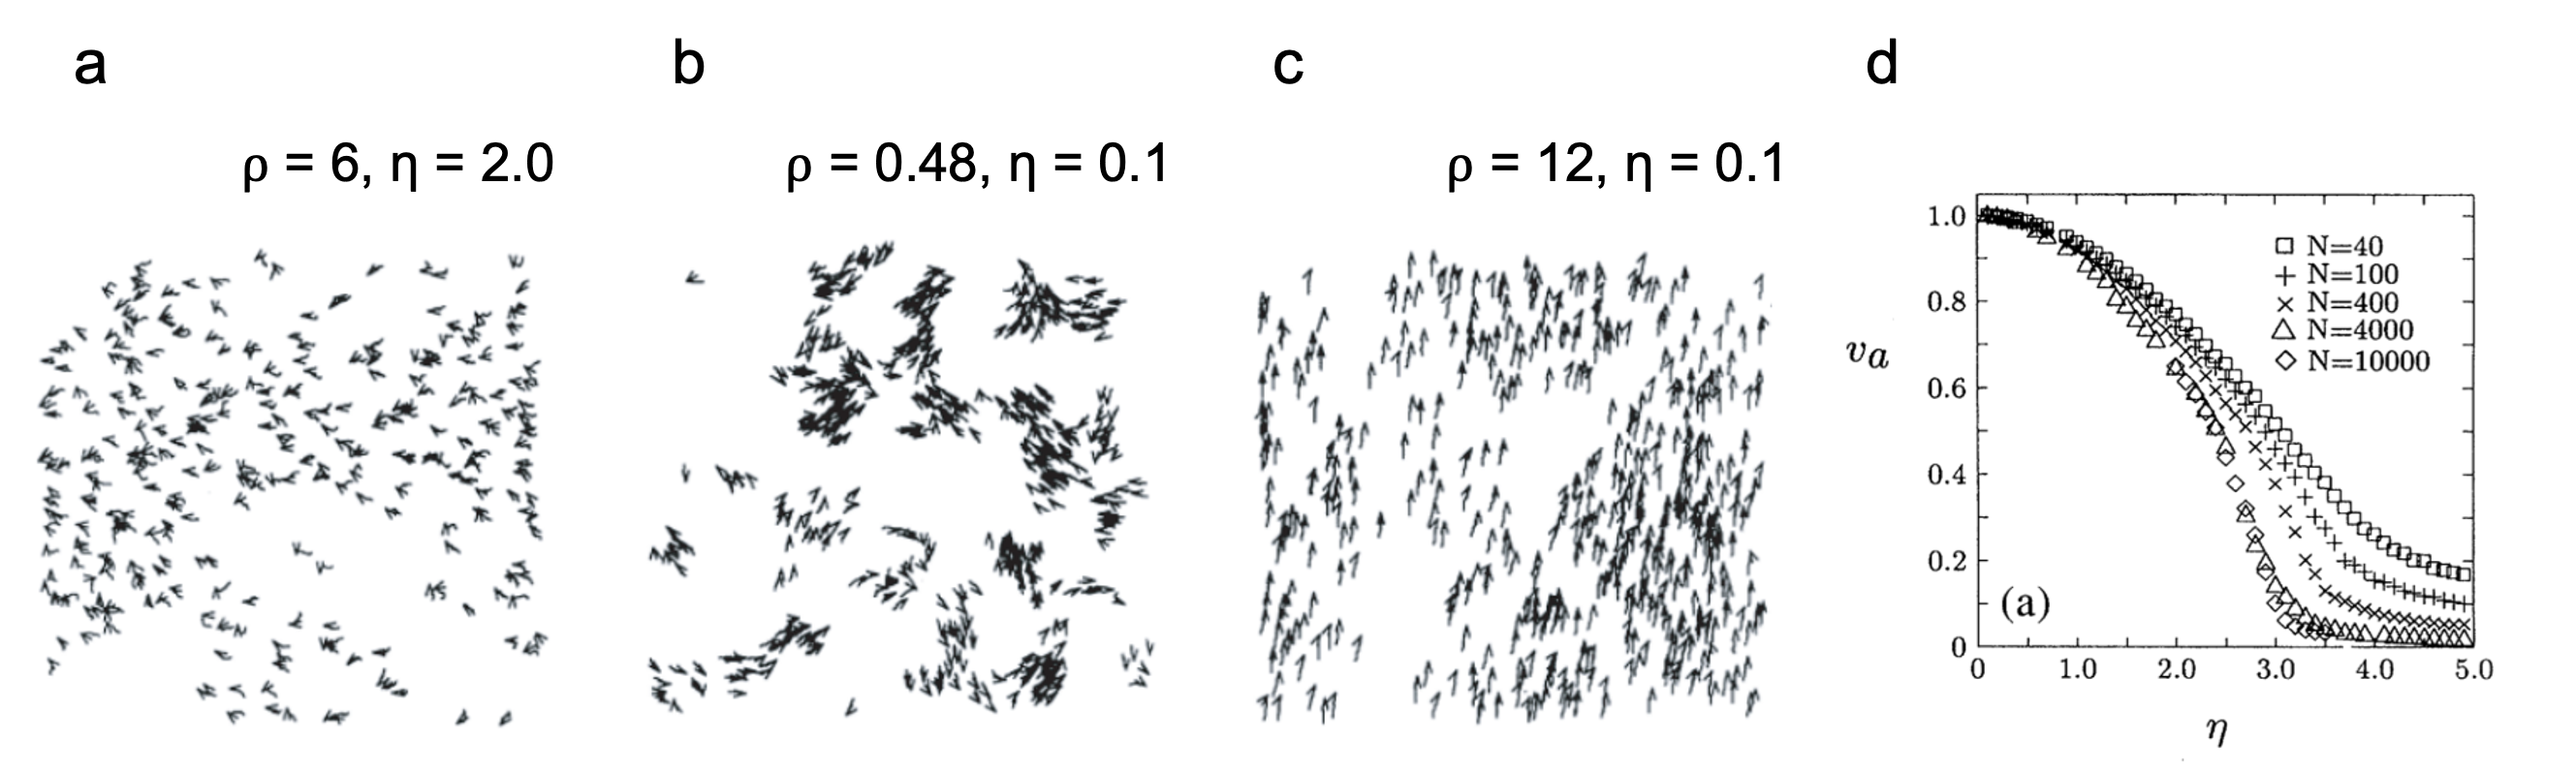
\includegraphics[width=\linewidth]{chapters/activeMatter/figsActiveMatter/figVicsek}
	\caption[Vicsek model]{Vicsek model: \textbf{a} State with random motion and low correlation. \textbf{b} Coherent motion in random directions. \textbf{c} Polar alignment dominates motion in a spontaneous direction. \textbf{d} Evolution of the average velocity as a function of the noise demonstrates the presence of a kinetic phase transition.}
	\label{fig:Vicsek}
\end{figure*}



Further developments in the physical description of flocking systems were introduced by Toner and Tu \cite{toner1995,toner1998}. Where a hydrodynamical approach yielded a continuum model of coarse-grained density and velocity fields \cite{toner2005}. This was followed by a kinetic theory derivation of the Toner and Tu equations by Bertin et al. \cite{bertin2006}, demonstrating that coarse-graining of the Vicsek model leads to a microscopic foundation for the hydrodynamical theory. This phenomenological approach allowed for the description of large-scale, and long-time fluids of flocking active units.




\textit{Collective motion in real biological systems ---} The introduction of these models naturally led to the study of real life biological systems that exhibit flocking behaviour and assessments as to the validity of the predictions of these theories.  
One such study approached this through the tracking of real-life flocking birds, from which the coordinates of the flock and underlying dynamics were compared with the predictions of hydrodynamic theory \cite{cavagna2014}. The study found that when examining the individual diffusion of the birds, the movement was both super-diffusive and anisotropic; in agreement with Toner and Tu. Furthermore, it was shown that the individuals in the flock would interact with the same number of neighbours regardless of the density (in this case seven) \cite{ballerini2008}. Similar methodologies and analysis have been applied to systems of swimming fish \cite{gautrais2009}, locust migratory bands \cite{bazazi2008}, and bacterial colonies \cite{zhang2010b}.


\textit{Collective motion in model experimental systems---} while the observation and measurement of real-life flocking systems is crucial in developing an understanding to the physics governing these systems; these biological realisations are highly complex and feature many overlapping interactions that make comparison with theoretical predictions difficult. To address this issue, many model systems have been designed to study the physics of collective motion without additional long-range interactions or unwanted features, and where the included interactions are well understood. 
One such system involves an ensemble of individual disks designed with a built-in polar asymmetry. These disks are arranged in a monolayer upon a vibrating platform, causing them to move quasi-ballistically with a large persistence length and demonstrating the onset of collective motion \cite{deseigne2010}. Another study observed the emergence of collective motion through a highly dense system of actin filaments propelled on a bed of molecular motors \cite{schaller2010}. These filaments become coherently organised and display a plethora of long-range polar structures including clusters, swirls and bands.
Collective motion has also been observed in active colloidal systems. 
Through a mechanism known as induced-charge electrophoresis, colloidal Janus particles are propelled when exposed to an alternating electric field \cite{gangwal2008}. As a function of the frequency of this field, the particles exhibit a range of collective behaviours such as swarming, flocking and motile particle chains \cite{yan2016}.


%Through a mechanism called 'Quinke rotation' colloids are rolled across a substrate when exposed to an electric field. As well as providing a propulsion mechanism, the electric field creates hydrodynamical flows around the particles that promote alignment at short distance, producing a system of self-propelling particles with a polar alignment. \cite{bricard2013}. This system of microscopic particles has been instrumental in the study of macroscale collective motion  and has proven to be amenable to computational modeling also \cite{geyer2019,mauleonamieva2020,lu2018,pradillo2019,bricard2015,mauleon-amieva2021}.


\textit{Collective motion with nematic alignment ---} thus far we have only considered polar alignment. However, there exist some systems; such as elongated bacteria \cite{peruani2012}, where the geometry dominates the alignment interactions. In these systems, particles can either align or anti-align depending on the angle between them. A kinetic theory was presented for a system of self-propelling rods by Baskaran et al \cite{baskaran2008}, and extended to a set of nonlinear field equations from a nematic Vicsek model by Peshkov et al \cite{peshkov2012}. These systems feature collective motion phenomena unique to systems with nematic alignment in the form of bands (lanes) in which the individual units are aligned parallel along the band as it moves macroscopically \cite{chate2006,ginelli2010}. Bands have been observed experimentally in system of actin filaments which can exhibit both nematic bands and polar waves \cite{huber2018}.

  

\subsection{Motility induced phase separation}

We turn now to another dynamical phase unique to active matter systems. Here we discuss the resultant liquid-gas separation of self-propelling polar particles with \textit{scalar} interactions. The dynamics of these systems evolve as described by active Brownian motion or run and tumble dynamics, where interactions between the active units are purely repulsive or steric. First predicted analytically for a one-dimensional run and tumble system \cite{tailleur2008}, and then demonstrated in two-dimensional simulations of active Brownian particles \cite{fily2012, redner2013}, and later in three-dimensions \cite{stenhammar2014,wysocki2014}. The phenomena of active particles separating into dense and dilute phases as a result of persistent motion has become known as motility-induced phase separation (MIPS). An example of this is shown in Fig. \ref{fig:MIPS} where a system of  active Brownian disks demonstrate this liquid-gas coexistence.  
\begin{figure*}
	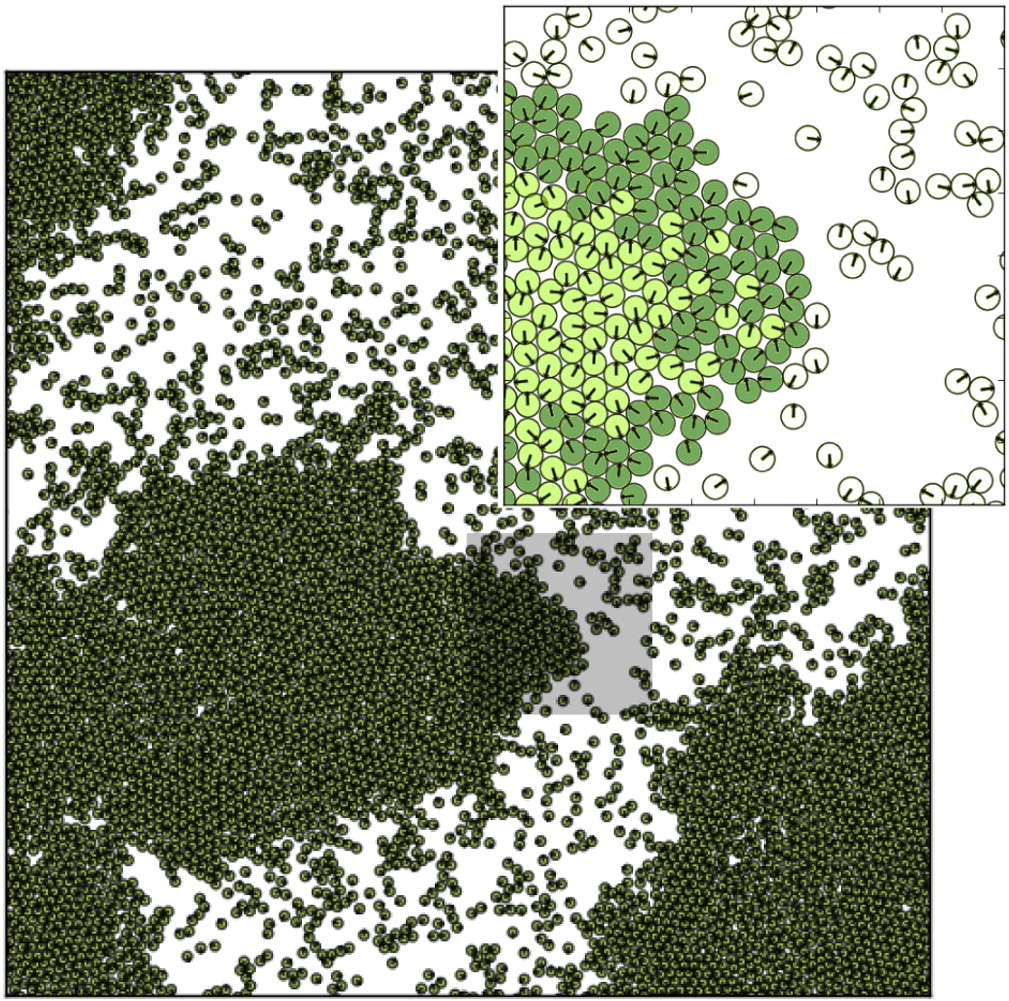
\includegraphics[width=0.5\linewidth]{chapters/activeMatter/figsActiveMatter/figMIPS}
	\centering
	\caption[Motility induced phase separation]{Motility-induced phase separation in a system of active Brownian disks. The wide view shows the coexistence of the dense liquid and the dilute gas in this non-equilibrium phase. The inset shows a closer view, where particles in the bulk liquid are coloured light green; particles on the boundary are coloured dark green; and particles in the gas phase are depicted in white. A line on each disk denotes the direction of self-propulsion. Reproduced from  ref. \cite{marchetti2016}.}
	\label{fig:MIPS}	
\end{figure*}
The principle mechanism responsible for this behaviour is now well understood \cite{cates2015}: self-propelling particles will aggregate where their motion is slowed, while at high density; movement is further slowed as a result of steric or biochemical interactions (such as quorum sensing \cite{miller2001}). These two factors compound, resulting in a density-dependant velocity that separates the system into dense and dilute fluid phases.
%One such biochemical interaction is that of  Quorum sensing. In bacterial suspensions, individual bacteria will count the number of bacteria in an area and slow down depending on the density \cite{miller2001}. 




\textit{MIPS in active Brownian particles ---} thanks to the simplicity of the system, active Brownian particles (ABP) have been the focus of many studies. Evidence for MIPS in systems of ABP have been shown with both hard-sphere potentials \cite{redner2013,bialke2013,stenhammar2013} and soft repulsive potentials \cite{fily2012,fily2014}. Unlike run and tumble bacterial systems, where the self-propulsion velocity has a defined density dependancy \cite{tailleur2008}; ABP  feature only excluded volume interactions. In these systems the particle slow-down and accumulation responsible for MIPS derives from particle collisions at high density. In this case it is reasonable to measure the average velocity of a particle $v (\rho)$ in the direction of the active propulsion \cite{cates2015}. In homogeneous systems of ABP this velocity $v(\rho)$ decreases as a function of $\rho$ with a near linear relationship \cite{fily2012,redner2013,stenhammar2014}:

\begin{equation}
	v(\rho)=v_{p}\left[1-\rho / \rho^{*}\right],
\end{equation}

\noindent where $v_p$ is the constant propulsion velocity, and $\rho^*$ is the density at which $v$ vanishes due to close packing. As well as confirmation via simulation, this relationship has been described with kinetic theories \cite{fily2012,fily2014,stenhammar2013}. Moreover, the decrease in motility from MIPS can be identified via the effective diffusion coefficient:

\begin{equation}
	D_{\textrm{eff}}(\rho)=v(\rho)^{2} \tau_R / d+D_{T},
\end{equation}

\noindent where $\tau_R$ is the rotational diffusion time, $d$ is the dimension, $D_T$ is the translational diffusion coefficient. Therefore, as $v(\rho)$  decreases as a function of density, so does the effective diffusion \cite{fily2012,fily2014,stenhammar2014}.


One important aspect of these systems that must be considered, is the contributions of the Brownian thermal fluctuations within the particle dynamics. These fluctuations can work to disrupt or inhibit MIPS, and therefore these systems are often described by a parameter known as the Péclet number: 

\begin{equation}
	\pecl = \frac{v_p}{\sigma D_R},
	\label{eq:pe}
\end{equation} 
 
 \noindent where $\sigma$ is the particle diameter. $\pecl$ relates the ratio of motility due to persistent motion ($v_p/D_r$) to the particle diameter $\sigma$. At high values of $\pecl$, motion is dominated by large persistent paths; while at low $\pecl$ motion more closely resembles Brownian motion. 
 Through analysis of the local density it is possible to determine the spinodal line of the MIPS phase \cite{digregorio2018,omar2021a}, where MIPS will not occur below a critical $\pecl_c$: where $Pe_c \simeq  18$ in two-dimensions and   $Pe_c \simeq  40$ in three-dimensions \cite{turci2021,digregorio2018,omar2021a}.  For systems of active Brownian particles, extensive work has been under taken to produce the full phase diagram in the $\pecl$ --- $\phi$ space, where $\phi $ is the volume fraction. The phase diagrams for active Brownian particles are reproduced in 2D and 3D in Fig. \ref{fig:2D_3D_phaseDiagram}a and Fig. \ref{fig:2D_3D_phaseDiagram}b respectively.
Both phase diagrams report liquid-gas coexistence of the MIPS phase within spinodal phase boundaries similar to those of the equilibrium phase diagram. It should be noted that these works use similar but alternate definitions for $\pecl$ to the one defined in eq. \ref{eq:pe}, however this only constitutes a small linear rescaling of the values. 
 
The MIPS region in both 2D and 3D broadens with increasing activity, and although both phase diagrams look qualitatively similar, there are some important distinctions. As we have already stated, the MIPS phase separation occurs at higher propulsion velocities in 3D than in 2D. This occurs as a result of the difference in reorientation time $\tau_R$ in the two cases, which for a system with a rotational diffusion coefficient $D_R$, the corresponding reorientation times are: $\tau_{R,2D} = 1/D_R$ and $\tau_{R,3D} = 1/2D_R$. Therefore, as the 2D timescale is twice that of the 3D case, the particles exhibit more persistent dynamics and are more likely to be blocked upon collision, leading to phase separation \cite{siebert2017}. Another significant difference in the MIPS phases between the two dimensionalities lies in the structure of the phase separation. In 2D, the MIPS topology is that of disconnected droplets of the dense phase within a matrix of the dilute phase. Whereas in 3D the phase transition occurs via the nucleation of a single domain of the dense phase \cite{stenhammar2014}.
Recent works \cite{omar2021a,turci2021}, haven shown that for active Brownian spheres the MIPS coexistence phase is only metastable, decaying at long-times through an ordering transition, and that in three-dimensions the MIPS phase is enclosed by gas-crystal coexistence. Finally, it should be mentioned that in systems with soft potentials, the MIPS boundary will shift depending of the steepness of said potential \cite{martin-roca2021}.

 
\begin{figure*}
	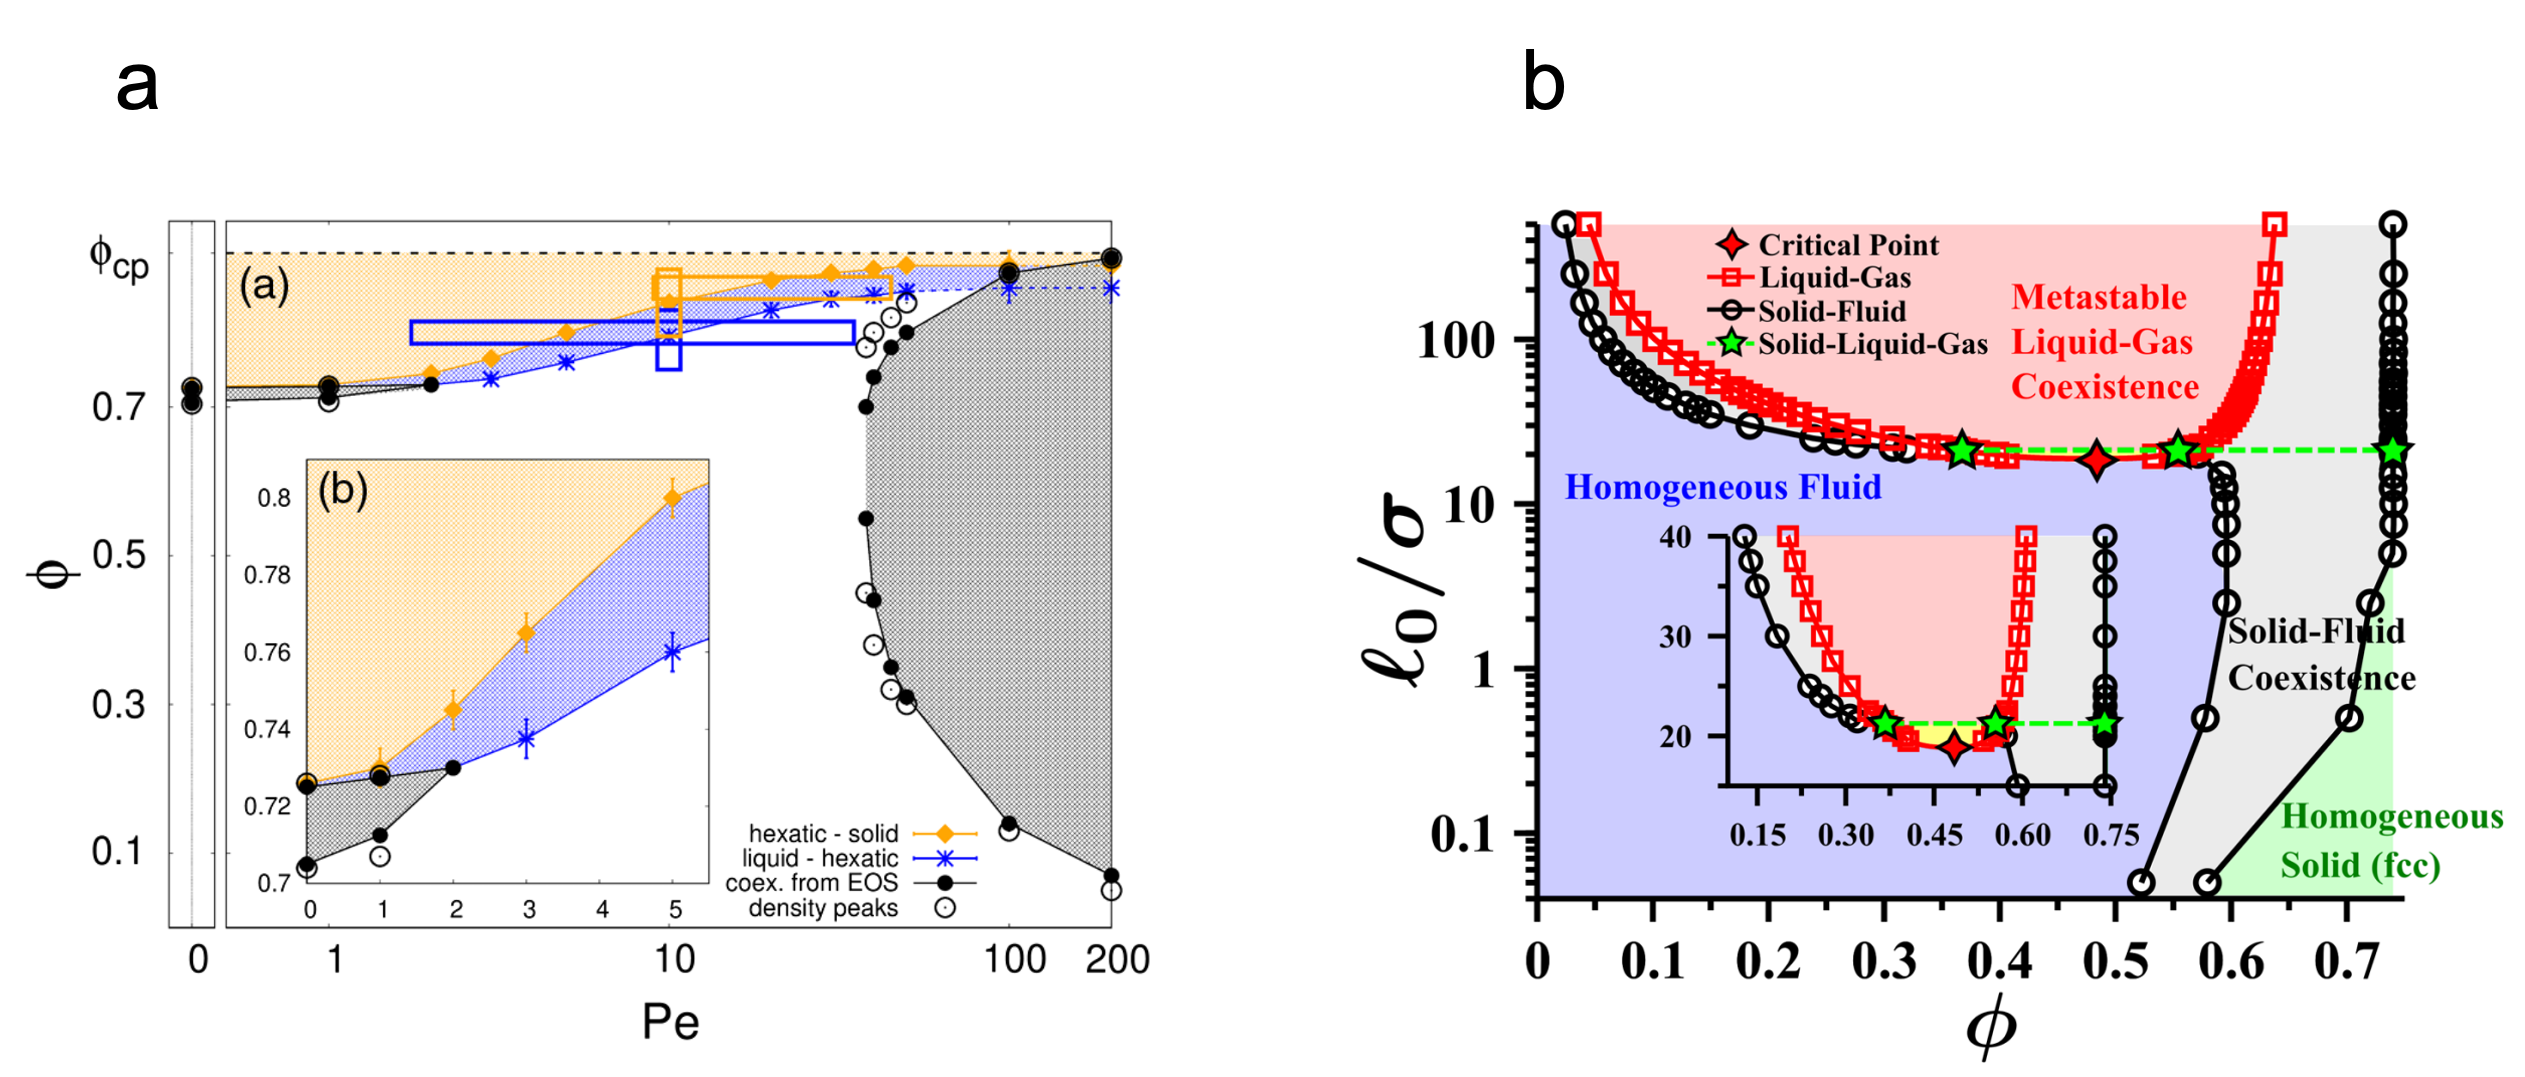
\includegraphics[width=\linewidth]{chapters/activeMatter/figsActiveMatter/figPhaseDiagrams}
	\centering
	\caption[Phase diagram of active Brownian particles]{\textbf{a} Phase diagram of active Brownian disks, reproduced from ref. \cite{digregorio2018}. \textbf{b} Phase diagram of active Brownian spheres, reproduced from ref. \cite{omar2021a}. Both phase diagrams possess a similarity with the equilibrium liquid-gas phase diagram. In 2D ABPs crystallise into a hexagonal lattice, while an FCC solid is reported in 3D.}
	\label{fig:2D_3D_phaseDiagram}	
\end{figure*}
 
 
\textit{MIPS in experimental systems ---} the observations of MIPS in simulated active systems prompted many studies in experimental model systems in search of this non-equilibrium phase transition. Several studies reported to have observed MIPS in experiment including systems of catalytic self-phoretic active colloids \cite{theurkauff2012}, light activated active colloids \cite{palacci2013}, and active Janus particles \cite{buttinoni2013}. These studies report coarsening clusters of colloids, claiming to have observed MIPS. However, today there is a general agreement that this is not MIPS (with a notable exception \cite{liu2019a}), as the particle density in these systems is far below the phase boundary, and propulsion speeds too low. 
Moreover, often the mechanisms which enable the self-propulsion of colloids bring with them additional interactions, such as alignment. A recent work, examined such a system of aligning active Janus particles \cite{vanderlinden2019}, in which a competition arises between the alignment and MIPS. 

\textit{Towards a thermodynamical understanding of MIPS ---} active matter provides a grouping of systems that are amenable to the study of non-equilibrium thermodynamics. The dilute and dense fluid coexistence of the  MIPS phase is strikingly similar to that of a first-order liquid gas transition in an equilibrium system. In fact multiple studies have focussed on mappings between the two \cite{tailleur2008,speck2014,cates2013,takatori2015}. 
Indeed, it has been shown that by including non-equilibrium contributions within equilibrium descriptions, such as a pressure equation of state; certain features of active brownian systems can be captured \cite{winkler2015,fodor2016a,levis2017}.
Indeed the question of pressure, and whether either a mechanical or local description is correct and whether or not it can be considered a state variable has garnered much interest \cite{speck2016,winkler2015,das2019,solon2015a,malgaretti2021,solon2015b}.  
%\todo{Be more specific}
A similar level of interest has attracted work into the surface tension of the MIPS dense phase \cite{solon2018,patch2018,lee2017}.


\subsection{Towards high density}

Another area within the field that has been a focus for recent study is that of active systems at very high densities. For disks and spheres the resultant high-density states depend on the size distribution: mono-disperse systems (uniform size distribution) at very high densities will crystallise; while in poly-disperse systems (where the units vary in size), the crystalline order is disrupted and instead the system trends towards an active glass.


\textit{Active crystals ---} regarding crystallisation in active systems, the key question is the following: How does the crystalline order compete with the physics of active matter?
The answer is not trivial. The freezing transition of active systems is shifted relative to their equilibrium counterpart, the nature of which cannot be described using effective temperature concepts \cite{loi2008,wang2011}.
The relationship between density and activity has been studied in the context of the phase diagrams: In 2D, active Brownian disks crystallise into a hexagonal lattice \cite{bialke2012,digregorio2018}; and in 3D, active spheres were reported to form crystals with the FCC polymorph \cite{turci2021,omar2021a}. In both cases the freezing line is found to move to higher area or volume fraction as a function of activity. In this sense, activity may be said to suppress crystallisation. This effect can be seen in the full phase diagrams of these systems reproduced in Fig. \ref{fig:2D_3D_phaseDiagram}. 

The influence of activity on the process of nucleation has been studied via classical nucleation theory, in which a renormalised surface tension was found to provide reasonable agreement with simulation \cite{redner2016}. One intriguing and unexpected effect of activity upon crystallisation was the observation of annealing of grain boundaries in the case of the addition of a small quantity of active particles to an otherwise passive system \cite{vandermeer2016}. Active particles with inertia will also crystallise in two-dimensions \cite{liao2021}, although this crystallisation is inhibited by the inertia with respect to active Brownian particles.
In experimental colloidal systems, self-propelling colloids with alignment driven through quinke rotation haven been observed forming \textit{amoebalike} motile crystallites \cite{mauleonamieva2020}. Furthermore, while the study of active colloids in three-dimensions is in its infancy; a system active multi-polar Janus colloids was observed exhibiting crystallisation into a variety of polymorphs \cite{sakai2020} .
Despite these efforts, there is still much to be understood with regards to the crystallisation of active particles, such as the difference in nucleation in active and equilibrium systems.


\textit{Active glasses ---} glasses constitute a condensed matter state in which the behaviour is like that of a solid, but contrary to crystals the microscopic structure of its units do not possess any long-range order. Creation of these materials usually involves compressing or supercooling a liquid whilst avoiding crystallisation. If the viscosity of the liquid reaches or exceeds a certain value (usually $10^{12}$Pa $s$), it can be considered to be an amorphous solid, or glass. This process, known as the glass transition carries the supercooled liquid out of equilibrium and into a unique non-ergodic state \cite{janssen2019}.
The study of glass has a long history, the first examples date back thousands of years, and the creation process has been understood for centuries. Interestingly, despite this all of this, the glass transition is ruled by a web of complex phenomena, of which a true understanding remains elusive \cite{berthier2011}. Some examples of phenomena responsible for glassy dynamics include: dynamic heterogeneity \cite{kawasaki2007}, extremely slow dynamics \cite{malins2013}, and \textit{fragility} \cite{sastry2001}.  



The surge of interest in active systems has prompted many studies of glassy active systems in search of new fundamental physics. Given the extreme timescales inherent to glass physics, many of these works have focused on  computational systems such as active Brownian particles:
 For example, in a system of soft active spheres, Wysocki et al. observed behaviour characteristic of the liquid phase at densities close to random close packing \cite{wysocki2014}.
Mandal et al. \cite{mandal2020,mandal2021} studied an active version of the Kob-Andersen mixture, where cage trapping in the active glass causes slower dynamics than a passive brownian glasses in the short-time, but faster than brownian dynamics in the long time regime. This non monotonic evolution of the relaxation was also found in a system of active Ornstein-Uhlenbeck particles by Szamel et al. \cite{szamel2015}, who also developed a mode-coupling-like theory for active glasses \cite{szamel2015,szamel2016}. 


Beyond these computational works, there is large body of work applying the ideas of active glasses physics to dense biological tissues. For example the dynamical slowdown and fragility in eukaryotic cells \cite{zhou2009}, dynamic heterogeneity in bacteria cytoplasm \cite{parry2014}, and epithelial cell sheets \cite{angelini2011}. The latter has inspired computational works with the employ of self-propelling vertex models to study glassy cell dynamics \cite{bi2016,bi2015}.


\textit{Collective Motion at high density ---} in section \ref{section:activeMatter:CollectiveMotion} we reviewed the collective motion phenomena arising from polar active particles with alignment interactions. These systems are rarely taken to extreme densities, however in these cases there is often an emergence of phenomena distinct to that of these systems at lower densities. For example, polar aligning disks that flock at low density will crystallise above a critical density \cite{briand2018a}. 
Active colloids with alignment and propulsion from quinke rotation assemble into roving flocks. Furthermore, when these flocks exceed a critical density: the colloids cease their collective motion, and jam into a solid phase, indicating that this density induced suppression of collective behaviour could be common to a broad range of active systems \cite{geyer2019}. Finally, in an interesting application of active matter methodologies, structural mechanisms governing high-density human crowds were revealed \cite{bottinelli2016}.


\section{Active matter in complex environments}
\label{section:activeMatter:confinement}

Up to this point, we have primarily considered active systems in unbounded, homogeneous environments. The bulk dynamics of active matter bring about a rich and complex set of phenomena, the study of which has led to a deeper fundamental understanding of non-equilibrium systems. However, in reality the real-life examples that inspire these systems do no exist with an absence of environment. On mesoscopic lengthscales, examples of real-life active units such as biological microswimmers exist in the crowded and complex environments within 
organic tissues \cite{hutmacher2000}, inside cells \cite{isermann2017}, and porous soils \cite{gannon1991}.
Therefore, in the following section, we focus on the interplay of persistent self-propulsion and the complex environments pertinent to active Brownian matter.

\textit{Interaction at a boundary ---} we begin with the simplest case: a particle interacting with a wall. With the introduction of a boundary, there is now an asymmetrical condition imposed on to the particle motion. A particle propelling towards a wall will collide and remain stuck at the boundary until the reorientation mechanism of the active direction changes to a sufficient angle from the boundary to escape. This asymmetry incurs wall accumulation of active particles resulting in particle configurations not observed in systems at equilibrium. This effect was first observed in bacterial systems where hydrodynamics play an essential role \cite{berke2008}. However, it was later proven that wall accumulation of active spheres will occur with purely repulsive interactions \cite{elgeti2013}.  
In addition to absorption at walls, active particles will tend to move along the surface of boundaries. This phenomena has been described with an effective force description, where a tangential component of the propulsion force, drives sliding motion along the boundary \cite{vanteeffelen2008}.

The combination of these accumulation and sliding behaviours produce interesting resultant phenomena at higher particle densities and in more complex environments. For example, active particles at sufficient density and activity will incur a complete wetting of a solid surface \cite{neta2021}. Capillary action has been observed for scalar active matter, where a liquid of dense active particles is drawn through a thin tube as a result of their activity \cite{wysocki2020}. The same system was observed demonstrating \textit{spontaneous imbibition}, where a wetting liquid is drawn into a porous medium \cite{wysocki2020}. The shape of boundaries is another important factor for these systems. In an experimental system of swimming bacteria; it was shown that entrapment of bacteria at curved boundaries was significantly reduced below a characteristic radius \cite{sipos2015}.
A recent work from Dor \etal \cite{dor2021} looked at the effect of disordered boundaries on scalar active matter. In this case the presence of the disordered boundary results in the destruction of bulk phase separation and the prevention of uniform wetting at the boundary.

\textit{Active dynamics on disordered landscapes ---} diffusion through disordered environments has been studied extensively in equilibrium systems. Studies focusing on model environments such as the Lorentz gas \cite{vanbeijeren1982}, which is comprised of randomly distributed spherical obstacles; has provided great insight into transport properties of random heterogeneous media \cite{dettmann2014}. The nature of the Lorentz gas is largely dependent on the density; over a certain threshold the system undergoes a percolation transition, where free space is no longer continuous through the system \cite{spanner2011}. The diffusion of active particles through this environment is heavily affected by the density of the obstacles: below percolation they perform the same subdiffusive dynamics as equilibrium systems, while reaching the long-time dynamics quicker. Above percolation the long-time diffusion is slower than passive systems as the persistent motion increases trapping \cite{zeitz2017}. 

Reichhardt and Olson-Reichhardt \cite{reichhardt2014,reichhardt2017,reichhardt2018a,reichhardt2018b} have extensively studied the dynamics of run and tumble particles on 2D landscapes with disordered fixed obstacles. In these systems an increase in the run length causes a non-monotonic response in the measured net transport. Initially they observe an increase in the average velocity but this reaches a maxima and then reduces as a result of cluster and crystallite formations jammed within the obstacles \cite{reichhardt2014}. At high obstacle and particle densities the system enters a \textit{pinned} state, where the combination of high density and fixed obstacles causes arrest in the active particle population \cite{reichhardt2018a}. As a function of density and activity the system undergoes a depinnning transition to a continuous flowing phase \cite{reichhardt2018b}. Furthermore, in the high density, high activity regime; the systems enters an intermittent state where depinning and motion occur in avalanches \cite{reichhardt2018b}.  
  

In a run and tumble system with diffusive obstacles, Bertrand \etal \cite{bertrand2018}, demonstrated an activity dependent non-monotonic diffusivity that shows potential for optimisation of run and tumble active matter in complex environments. In a similar system, Irani \etal \cite{irani2022} observed the influence of the obstacle density on bacterial reorientation, where the local geometry of the environment determines the optimal path. 
Moreover, in a disordered lattice of asymmetrical obstacles active particles exhibited a spontaneous inversion of the net particles current, opening avenues to possible control of these systems \cite{borba2020}.

 
 As well as computational studies, there have been several notable experimental realisations of active matter in disordered or patterned environments: in a system of active colloids propelling through a random lattice; the colloids experience smooth transitions from diffusive, to subdiffusive to localisation as a function of increasing obstacle density \cite{morin2017}. In this system, in addition to hard interactions, the colloids experience a repulsive electrostatic interaction with the obstacles, resulting in a slow down of the long-time diffusion. Biological microswimmer (microalga) observed swimming on an array of pillars, experience a decrease in their effective diffusion with increasing pillar density \cite{brun-cosme-bruny2019}. In a similar system with bacterial swimmers, the effective mean free path was determined to be the key geometrical parameter governing transport \cite{dehkharghani2022}. 
  
 
 \textit{Active matter in 3D complex environments ---} as a result of the experimental challenge that comes with the observation of three-dimensional active systems (especially in complex environments); this area is underdeveloped, with some noteworthy exceptions: a work from Bhattacharjee \etal \cite{bhattacharjee2019}, showed the first direct observation of bacteria swimming in 3D porous media. Interestingly, the dynamics were not found to feature simply run and tumble dynamics with run lengths reduced due to confinement, as is the common assumption. Instead, the environment places strong geometrical constraints where the bacteria will swim through directed paths determined by the confinement structure; or become transiently stuck in more confined spaces. These observations support the work done simulating active systems on disordered landscapes \cite{zeitz2017,reichhardt2014,bechinger2016a,reichhardt2018b}, showing that these complex environments incur changes to active dynamics beyond the simple rescaling of diffusion, drawing out fundamentally different behaviours. Modelling of this system was later shown to reproduce the observed directional persistence \cite{perez2021}.
 
% \textit{Sorting of active matter ---} using what we know to our advantage...
%  \fergus{corinna maas maze, ordered array in review}
% 


\section{Active Janus particles}
\label{section:activeMatter:janus}

For the final section of this chapter, we give special attention to active Janus colloids. A \textit{Janus} colloid usually refers to spherical particles of size nm to $\mu$m where each hemisphere features a unique and distinct surface chemistry \cite{zhang2017}. These particles can be made to undergo self-propulsion through a combination of particle surface modification and  control of the environment in which they inhabit. The application of these materials have experienced rapid expansion over the last decade, with the design and synthesis of many types of Janus particle. There are two primary mechanisms through which to induce self-propulsion of Janus particles: local energy conversion, and propulsion by external fields. While the propulsion of Janus particles via these two methods can be described by the same effective models \cite{bechinger2016a}, the difference between internal driving mechanisms and external driving mechanisms lies in the microscopic characteristics of the interactions with their environment \cite{bechinger2016a}.

\textit{Self-propulsion via local energy conversion ---} propulsion of Janus particles can arise from a number of energy sources (chemical, thermal, electrostatic), but they all rely on the creation of local gradients to generate self-phoretic motion.

\textit{Self-propulsion via external fields ---} directed motion of Janus particles can be induced through the application of alternating electric fields. This happens as a result of asymmetric liquid flows at the Janus particle surface. Motion via this mechanism is known as \textit{induced-charge electrophoresis} (ICEP) \cite{gangwal2008} and is the focus of the following section.

\subsection{Induced-charge electrophoresis (ICEP)}
First predicted theoretically by Dukhin and Shilov \etal \cite{dukhin1980,shilov2000}, popularised by Squires \etal \cite{squires2006}, and then later observed experimentally by Gangwal \etal \cite{gangwal2008}: ICEP refers to a mechanism that can facilitate motion in asymmetric particles as a result of unbalanced liquids flows at the particle surface. 
For propulsion by ICEP, the Janus colloid must be designed to possess two hemispheres of differing conductance or polarisability. This is often achieved by masking a layer of metal such as gold or chromium on to one hemisphere of a dielectric colloid such as silica or polystyrene. The result is a colloidal particle with anisotropic electrical properties. A further condition necessary for ICEP requires the suspension of the particles within an aqueous solvent. Aqueous solvents are composed predominantly of water and are thus soluble to electrolytes, through which the solvent can conduct electric currents. 


\begin{figure}
    \centering
    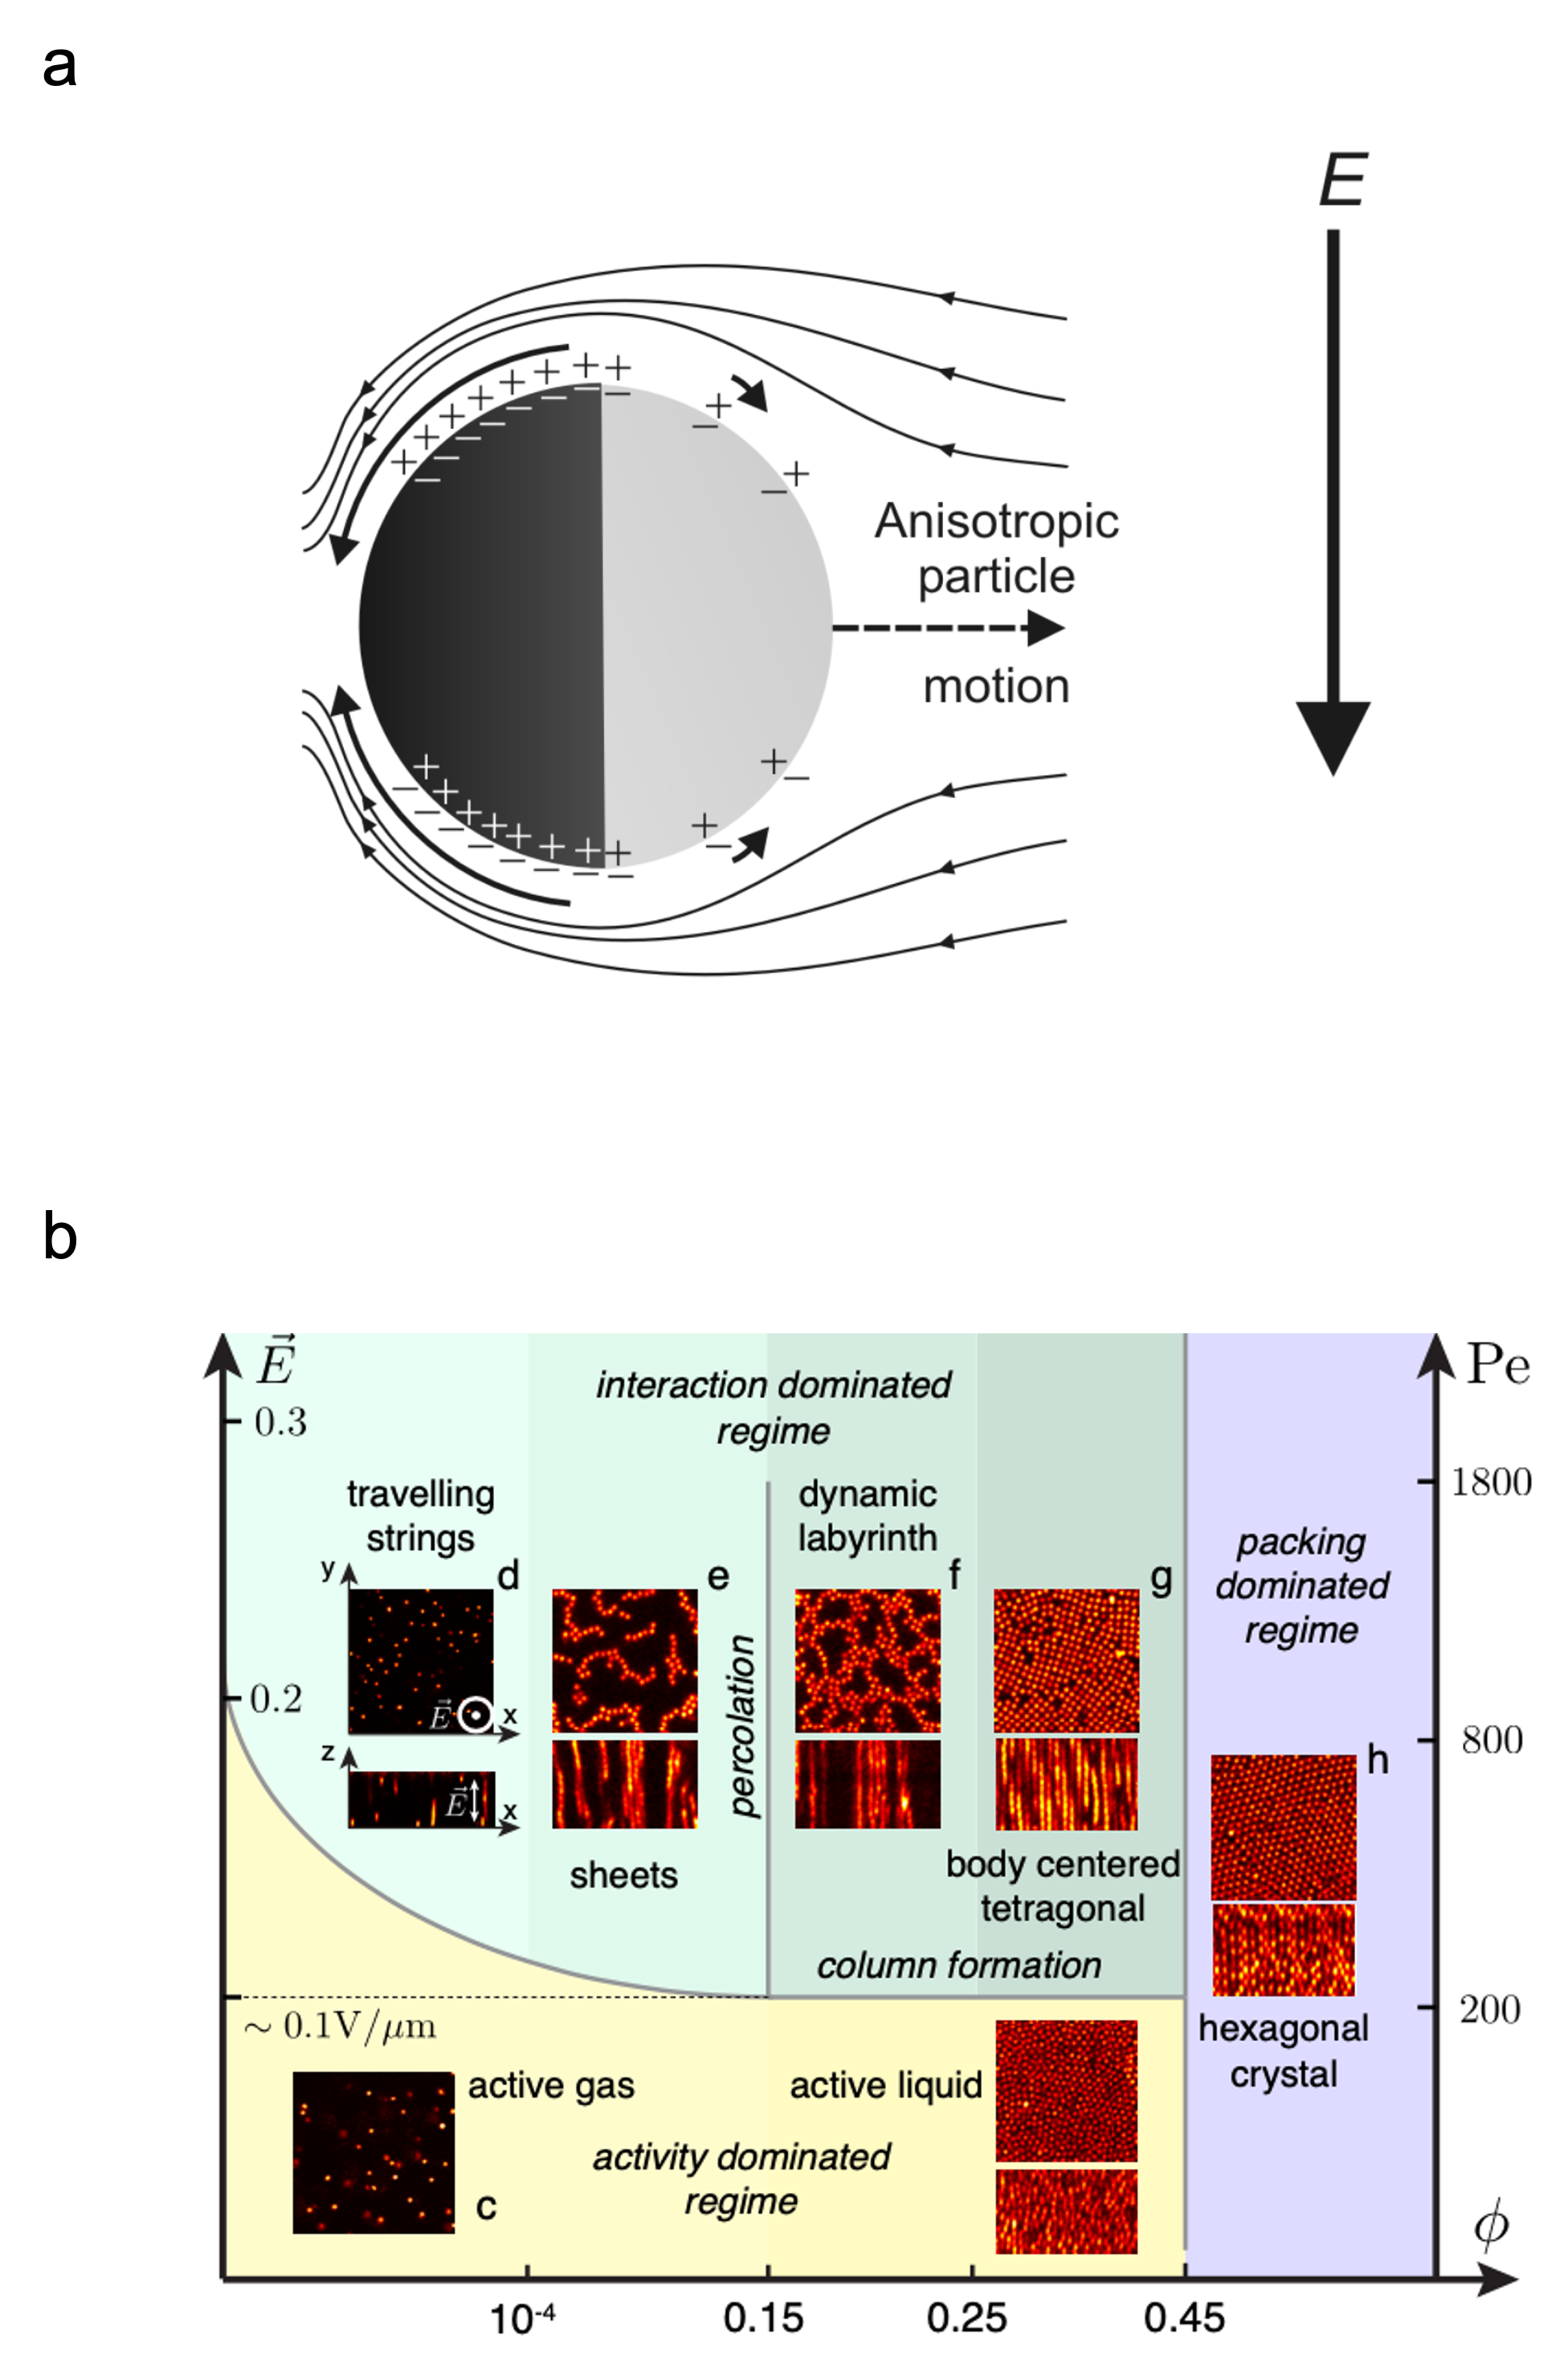
\includegraphics[width=0.7\linewidth]{chapters/activeMatter/figsActiveMatter/figJanusPhaseDiagram}
    \caption[Janus particles and induced-charge electrophoresis.]{\textbf{a} Schematic of a metallodielectric Janus particle undergoing phoretic motion via ICEP during one half cycle of the ac field. The electric double layer at the surface of the metallic hemisphere holds a greater polarisation than that of the dielectric hemisphere, and thus drives stronger electro-osmotic flows. The asymmetric distribution of these liquid flows at the particle surface result in ICEP motion away from the metallic hemisphere. Reproduced from ref. \cite{gangwal2008}. \textbf{b} Phase behaviour of active ICEP Janus particles. Reproduced from ref.  \cite{sakai2020}.}
    \label{fig:janus_pd}
\end{figure}

A suspension of metallodielectric Janus particles in an aqueous solvent will undergo self-propulsion via ICEP when exposed to an alternating electric field. This process is depicted in the schematic in Fig. \ref{fig:janus_pd}a for one half-cycle of the electric field. 
In the system depicted, a uniform electric field arises from a pair of parallel plates above and below the particle suspension. Upon the initialisation of the electric field, a current flows through the aqueous solvent between the plate electrodes. This current causes a redistribution of charge in the Janus particle from a random configuration to polarised configuration. Driven by the current, negative charges are drawn into a thin layer at one side of the particle, while positive charges act conversely, inducing an equal and opposite surface charge \cite{daghighi2011}. These surface charges attract counter ions in the surrounding solvent creating an electric double layer.
The ions in this induced dipolar double layer are subject to body forces from the applied electric field, where along with the liquid, they are driven into motion (electroosmosis). 
Due to the variation in the local surface charge across the asymmetric particle, the velocities of the electroosmotic flows change their value and direction.
Therefore, as a result of the differing conductance of the two hemispheres the ionic flows at the particle surface are unbalanced causing electrophoretic motion of the particle.

The propulsion velocity of these active Janus particles was predicted by Squires \etal \cite{squires2006} as $U_{\mathrm{ICEP}} \propto E_{0}^2$ where $E_0$ is the amplitude of the electric field. This has since been confirmed in experiment \cite{gangwal2008}.
As the ac field oscillates, the induced charges depicted in Fig. \ref{fig:janus_pd}a continually reconfigure in phase with the field, resulting in the uninterrupted unbalanced flows that drive motion, with velocities scaling with $E^2$.



\subsection{Phase behaviour of active ICEP Janus particles}
Active ICEP Janus particles in the dilute limit or at low field field strength, exhibit behaviour similar to active Brownian particles. In a system with the electric field aligned with the $z$ axis, the induced ionic flows propel the particle in the $xy$ plane. These propelling spherical particles are subject to rotational diffusion and thus the direction of propulsion will evolve diffusively like an active Brownian particle. Parallel to the field, there are no net solvent flows around the particle and so motion follows Brownian motion under gravity in this plane. It is for these dynamical characteristics that ICEP was chosen as the propulsion method for the experimental arm of this thesis. The main advantages being: the propulsion occurs in the bulk solvent rather than requiring a surface; and the similarity of  ICEP to active Brownian models allows for comparison of experimental observations with the wide body of work using the ABP model. 

In addition to propulsion, the electric field induces dipolar interactions between particles, a phenomena also observed for homogeneous colloids in the presence of external fields \cite{hynninen2005}. These dipoles are induced as a result of a mismatch between the dielectric constants of the colloids and the surrounding solvent. While homogeneous particles acquire a single dipole \cite{hynninen2005}, the dielectric response of Janus particles leads to separate dipole moments in each hemisphere \cite{yan2016}.
The phase behaviour of active Janus particles with dipolar interactions were the focus of a work from Sakai \etal \cite{sakai2020}. The phase diagram resulting from this work is reproduced in Fig. \ref{fig:janus_pd}b.


Here, they observe three dynamical behavioural categories: particles in the activity dominated regime behave similarly to active Brownian particles. This is a regime of low electric field strength and thus dipole interactions are weak and the colloids exhibit hard-sphere-like  interactions. At higher field strength, the behaviour of the ensemble is dominated by the dipole-dipole interactions. There are a number of emergent dynamical phases dependant on the volume fraction such as: two-dimensional \textit{sheets} where chains of particles aligned with the field come together to form larger structures;  a \textit{dynamic labyrinth}, where sheets come together in a percolating 3D structure; and at higher volume fraction the system crystallises into a tetragonal polymorph. Finally, in the packing dominated regime, the system solidifies into hexagonal crystalline structures.




